% Practice Test 23 — Florida Edition
% Questions: 30 (15 MC + 15 SA)
% Generated by scripts/generate_practice_tests.py

\begin{practiceQuestion}{1-3-q05}{mc}
\begin{questionText}
A car travels at a constant speed. It goes $150$ miles in $2.5$ hours. What is the constant of proportionality?
\end{questionText}
\choiceA{$30$ mph}
\choiceB{$60$ mph}
\choiceC{$75$ mph}
\choiceD{$150$ mph}
\correctAnswer{B}
\explanation{$k = \frac{150}{2.5} = 60$ miles per hour.}
\end{practiceQuestion}

\begin{practiceQuestion}{1-6-q30}{gsa}
\begin{questionText}
The table shows how many batches of muffins a bakery can make and the total flour used. How many cups of flour are needed for $15$ batches?

\begin{center}
\begin{tabular}{|c|c|}
\hline
\textbf{Batches} & \textbf{Flour (cups)} \\ \hline
$3$ & $7\frac{1}{2}$ \\ \hline
$6$ & $15$ \\ \hline
$9$ & $22\frac{1}{2}$ \\ \hline
$15$ & $?$ \\ \hline
\end{tabular}
\end{center}
\end{questionText}
\correctAnswer{$37\frac{1}{2}$ cups}
\explanation{$k = \frac{7.5}{3} = 2.5$ cups per batch. For $15$ batches: $2.5 \times 15 = 37.5 = 37\frac{1}{2}$ cups.}
\end{practiceQuestion}

\begin{practiceQuestion}{2-1-q21}{sa}
\begin{questionText}
$56$ is $80\%$ of what number?
\end{questionText}
\correctAnswer{$70$}
\explanation{Divide: $56 \div 0.80 = 70$.}
\end{practiceQuestion}

\begin{practiceQuestion}{2-2-q14}{mc}
\begin{questionText}
$27$ out of $180$ students earned an A on the exam. What percent earned an A?
\end{questionText}
\choiceA{$12\%$}
\choiceB{$15\%$}
\choiceC{$18\%$}
\choiceD{$27\%$}
\correctAnswer{B}
\explanation{$\frac{27}{180} = \frac{p}{100}$. Cross-multiply: $180p = 2700$. Divide: $p = 15\%$.}
\end{practiceQuestion}

\begin{practiceQuestion}{2-6-q22}{sa}
\begin{questionText}
You earned $\$180$ in interest on $\$2{,}000$ over $3$ years. What was the interest rate?
\end{questionText}
\correctAnswer{$3\%$}
\explanation{$180 = 2{,}000 \times r \times 3$ → $180 = 6{,}000r$ → $r = 0.03 = 3\%$.}
\end{practiceQuestion}

\begin{practiceQuestion}{2-7-q28}{gmc}
\begin{questionText}
The number line below shows an estimated value and an actual value. What is the percent error?

\begin{center}
\begin{tikzpicture}[scale=0.6]
  \draw[thick,->] (-0.5,0) -- (11,0);
  \foreach \x/\lab in {0/0,2/10,4/20,6/30,8/40,10/50} {
    \draw (\x,0.15) -- (\x,-0.15) node[below,font=\small] {\lab};
  }
  % Actual at 40
  \filldraw[funGreen] (8,0) circle (4pt);
  \node[above,font=\small,funGreen!80!black] at (8,0.3) {Actual: $40$};
  % Estimated at 35
  \filldraw[funRed] (7,0) circle (4pt);
  \node[below=10pt,font=\small,funRed] at (7,-0.15) {Estimated: $35$};
  % Arrow showing difference
  \draw[thick,<->,funOrange] (7,0.7) -- (8,0.7) node[midway,above,font=\small]{$5$};
\end{tikzpicture}
\end{center}
\end{questionText}
\choiceA{$5\%$}
\choiceB{$10\%$}
\choiceC{$12.5\%$}
\choiceD{$14.3\%$}
\correctAnswer{C}
\explanation{$\frac{|35-40|}{40} \times 100 = \frac{5}{40} \times 100 = 12.5\%$.}
\end{practiceQuestion}

\begin{practiceQuestion}{3-2-q15}{mc}
\begin{questionText}
What is $(-25) + 13 + (-8)$?
\end{questionText}
\choiceA{$-20$}
\choiceB{$-46$}
\choiceC{$30$}
\choiceD{$-4$}
\correctAnswer{A}
\explanation{$(-25) + 13 = -12$. Then $(-12) + (-8) = -20$.}
\end{practiceQuestion}

\begin{practiceQuestion}{3-3-q13}{mc}
\begin{questionText}
Death Valley's lowest point is $-282$ feet. A nearby hill is $134$ feet above sea level. What is the difference in elevation?
\end{questionText}
\choiceA{$148$ feet}
\choiceB{$-148$ feet}
\choiceC{$416$ feet}
\choiceD{$-416$ feet}
\correctAnswer{C}
\explanation{Difference $= 134 - (-282) = 134 + 282 = 416$ feet.}
\end{practiceQuestion}

\begin{practiceQuestion}{4-4-q08}{mc}
\begin{questionText}
Factor $24x - 16$.
\end{questionText}
\choiceA{$4(6x - 4)$}
\choiceB{$8(3x - 2)$}
\choiceC{$2(12x - 8)$}
\choiceD{$6(4x - 2)$}
\correctAnswer{B}
\explanation{GCF of $24$ and $16$ is $8$. Factor: $24x \div 8 = 3x$ and $-16 \div 8 = -2$. Result: $8(3x - 2)$.}
\end{practiceQuestion}

\begin{practiceQuestion}{4-5-q25}{sa}
\begin{questionText}
Simplify $(2x + 3) + (4x - 1) - (x + 5)$.
\end{questionText}
\correctAnswer{$5x - 3$}
\explanation{Combine: $2x + 3 + 4x - 1 - x - 5$. Variable: $2x + 4x - x = 5x$. Constants: $3 - 1 - 5 = -3$. Result: $5x - 3$.}
\end{practiceQuestion}

\begin{practiceQuestion}{5-3-q27}{gmc}
\begin{questionText}
The diagram shows two equal groups. Which equation represents this, and what is $x$?

\begin{center}
\begin{tikzpicture}[scale=0.6]
  % Group 1
  \draw[thick,fill=funBlue!20,rounded corners] (-0.5,-0.5) rectangle (3.5,2.5);
  \node[draw,fill=funBlue!40,minimum size=0.6cm] at (0.5,1.5) {$x$};
  \node at (1.5,1.5) {$+$};
  \node[draw,fill=funOrange!40,minimum size=0.6cm] at (2.5,1.5) {$4$};
  \node at (1.5,0.2) {Group 1};
  % Group 2
  \draw[thick,fill=funBlue!20,rounded corners] (5,-0.5) rectangle (9,2.5);
  \node[draw,fill=funBlue!40,minimum size=0.6cm] at (6,1.5) {$x$};
  \node at (7,1.5) {$+$};
  \node[draw,fill=funOrange!40,minimum size=0.6cm] at (8,1.5) {$4$};
  \node at (7,0.2) {Group 2};
  % Total
  \draw[decorate,decoration={brace,amplitude=8pt}] (9.2,2.7) -- (9.2,-0.7);
  \node[right] at (9.5,1) {$= 22$};
\end{tikzpicture}
\end{center}
\end{questionText}
\choiceA{$2(x + 4) = 22$, $x = 7$}
\choiceB{$2x + 4 = 22$, $x = 9$}
\choiceC{$x + 8 = 22$, $x = 14$}
\choiceD{$2(x + 4) = 22$, $x = 3$}
\correctAnswer{A}
\explanation{Two identical groups of $(x + 4)$: $2(x + 4) = 22$. Divide by $2$: $x + 4 = 11$. Subtract $4$: $x = 7$.}
\end{practiceQuestion}

\begin{practiceQuestion}{5-4-q10}{mc}
\begin{questionText}
Solve $\dfrac{x}{6} - \dfrac{2}{3} = \dfrac{1}{2}$.
\end{questionText}
\choiceA{$x = 3$}
\choiceB{$x = 7$}
\choiceC{$x = -1$}
\choiceD{$x = 10$}
\correctAnswer{B}
\explanation{Multiply every term by $6$: $x - 4 = 3$. Add $4$: $x = 7$. Check: $\frac{7}{6} - \frac{2}{3} = \frac{7}{6} - \frac{4}{6} = \frac{3}{6} = \frac{1}{2}$ \checkmark.}
\end{practiceQuestion}

\begin{practiceQuestion}{5-5-q24}{sa}
\begin{questionText}
Solve $\dfrac{x}{2} + 7 \leq 12$.
\end{questionText}
\correctAnswer{$x \leq 10$}
\explanation{Subtract $7$: $\frac{x}{2} \leq 5$. Multiply by $2$: $x \leq 10$.}
\end{practiceQuestion}

\begin{practiceQuestion}{5-6-q30}{gsa}
\begin{questionText}
A student has test scores of $78$, $85$, and $90$. She needs an average of at least $85$ on four tests to earn an A. Solve the inequality to find the minimum score $s$ on the fourth test, and describe the graph.

\begin{center}
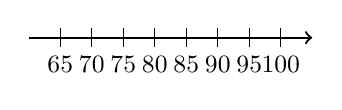
\begin{tikzpicture}[scale=0.08]
  \draw[thick,->] (60,0) -- (105,0);
  \foreach \x in {65,70,...,100} {
    \draw (\x,1.5) -- (\x,-1.5) node[below,font=\small] {$\x$};
  }
\end{tikzpicture}
\end{center}
\end{questionText}
\correctAnswer{$s \geq 87$; closed circle at $87$, shade right}
\explanation{$\frac{78 + 85 + 90 + s}{4} \geq 85$. Multiply by $4$: $253 + s \geq 340$. Subtract $253$: $s \geq 87$. Closed circle at $87$, shade right.}
\end{practiceQuestion}

\begin{practiceQuestion}{6-2-q22}{sa}
\begin{questionText}
A floor plan uses $1$ cm $= 6$ ft. On this plan, a room is $9$ cm long. On a second plan, the same room is $3$ cm long. What scale does the second plan use?
\end{questionText}
\correctAnswer{$1$ cm $= 18$ ft}
\explanation{Actual length: $9 \times 6 = 54$ ft. New scale: $54 \div 3 = 18$ ft per cm.}
\end{practiceQuestion}

\begin{practiceQuestion}{6-4-q25}{sa}
\begin{questionText}
A triangle has angles $60°$, $60°$, and $60°$, and one side measures $10$ cm. How many triangles can be drawn?
\end{questionText}
\correctAnswer{Exactly one}
\explanation{AAA alone gives many, but specifying a side length fixes the size. A triangle with all $60°$ angles is equilateral, so all sides are $10$ cm. Exactly one triangle.}
\end{practiceQuestion}

\begin{practiceQuestion}{6-5-q21}{sa}
\begin{questionText}
What shape is the cross-section when a cone is sliced vertically through its apex?
\end{questionText}
\correctAnswer{A triangle}
\explanation{A vertical slice through the apex of a cone produces an isosceles triangle. The base of the triangle is a diameter of the cone's base.}
\end{practiceQuestion}

\begin{practiceQuestion}{6-6-q11}{mc}
\begin{questionText}
Which statement about vertical angles is always true?
\end{questionText}
\choiceA{They are supplementary}
\choiceB{They are complementary}
\choiceC{They are equal}
\choiceD{They sum to $360°$}
\correctAnswer{C}
\explanation{Vertical angles are always equal. They are formed by two intersecting lines, and the opposite angles are congruent.}
\end{practiceQuestion}

\begin{practiceQuestion}{7-1-q22}{sa}
\begin{questionText}
The circumference of a circle is $62.8$ cm. Using $\pi \approx 3.14$, find the radius.
\end{questionText}
\correctAnswer{$10$ cm}
\explanation{$d = C \div \pi = 62.8 \div 3.14 = 20$ cm. Then $r = 20 \div 2 = 10$ cm.}
\end{practiceQuestion}

\begin{practiceQuestion}{7-5-q28}{gmc}
\begin{questionText}
The diagram shows a triangular prism. What is its total surface area?

\begin{center}
\begin{tikzpicture}[scale=0.4]
  % Front triangle
  \draw[thick,funBlue,fill=funBlue!10] (0,0) -- (6,0) -- (3,4) -- cycle;
  % Back triangle (offset)
  \draw[thick,funBlue,fill=funBlue!20] (2,1.5) -- (8,1.5) -- (5,5.5) -- cycle;
  % Connecting edges
  \draw[thick,funBlue] (0,0) -- (2,1.5);
  \draw[thick,funBlue] (6,0) -- (8,1.5);
  \draw[thick,funBlue] (3,4) -- (5,5.5);
  % Labels
  \node[below] at (3,0) {$6$ cm};
  \node[left] at (1.2,2) {$5$ cm};
  \node[right] at (4.8,2) {$5$ cm};
  \node[right] at (8,3.5) {$8$ cm};
  \node[above left] at (1,0.8) {$h = 4$ cm};
\end{tikzpicture}
\end{center}
\end{questionText}
\choiceA{$104$ cm$^2$}
\choiceB{$128$ cm$^2$}
\choiceC{$152$ cm$^2$}
\choiceD{$160$ cm$^2$}
\correctAnswer{C}
\explanation{Two triangles: $2 \times \frac{1}{2} \times 6 \times 4 = 24$ cm$^2$. Three rectangles: $6 \times 8 + 5 \times 8 + 5 \times 8 = 48 + 40 + 40 = 128$ cm$^2$. Total: $24 + 128 = 152$ cm$^2$.}
\end{practiceQuestion}

\begin{practiceQuestion}{7-6-q23}{sa}
\begin{questionText}
A rectangular prism has a volume of $360$ cm$^3$. Its length is $12$ cm and its height is $5$ cm. What is its width?
\end{questionText}
\correctAnswer{$6$ cm}
\explanation{$360 = 12 \times w \times 5 = 60w$. $w = 360 \div 60 = 6$ cm.}
\end{practiceQuestion}

\begin{practiceQuestion}{7-7-q02}{mc}
\begin{questionText}
Which formula gives the volume of a cylinder?
\end{questionText}
\choiceA{$V = 2\pi rh$}
\choiceB{$V = \pi r^2 h$}
\choiceC{$V = \pi r^2$}
\choiceD{$V = \frac{1}{3}\pi r^2 h$}
\correctAnswer{B}
\explanation{The volume of a cylinder is $V = \pi r^2 h$ (area of the circular base times the height).}
\end{practiceQuestion}

\begin{practiceQuestion}{8-1-q03}{mc}
\begin{questionText}
Which sampling method is most likely to produce a representative sample of a school's students?
\end{questionText}
\choiceA{Survey students in the cafeteria during lunch}
\choiceB{Survey every fifth student on an alphabetical class list}
\choiceC{Survey students who volunteer to participate}
\choiceD{Survey only students in honors classes}
\correctAnswer{B}
\explanation{Selecting every fifth student from a list is systematic and gives all students an equal chance, making it more representative.}
\end{practiceQuestion}

\begin{practiceQuestion}{8-3-q21}{sa}
\begin{questionText}
Data set: $4, 6, 7, 8, 10$. The mean is $7$. Find the MAD.
\end{questionText}
\correctAnswer{$1.6$}
\explanation{Deviations from mean: $|4-7|+|6-7|+|7-7|+|8-7|+|10-7| = 3+1+0+1+3 = 8$. MAD $= \frac{8}{5} = 1.6$.}
\end{practiceQuestion}

\begin{practiceQuestion}{8-4-q22}{sa}
\begin{questionText}
Group X: mean $45$, MAD $6$. Group Y: mean $57$, MAD $6$. Express the difference in means as a multiple of MAD.
\end{questionText}
\correctAnswer{$2$ MADs}
\explanation{Difference: $57 - 45 = 12$. In MADs: $\frac{12}{6} = 2$.}
\end{practiceQuestion}

\begin{practiceQuestion}{8-5-q05}{mc}
\begin{questionText}
How many total data values are in this stem-and-leaf plot?

\begin{center}
\begin{tabular}{r|l}
\textbf{Stem} & \textbf{Leaf} \\
\hline
$4$ & $2\;\;5\;\;8$ \\
$5$ & $0\;\;3\;\;3\;\;6\;\;9$ \\
$6$ & $1\;\;4$
\end{tabular}
\end{center}
\end{questionText}
\choiceA{$3$}
\choiceB{$8$}
\choiceC{$10$}
\choiceD{$15$}
\correctAnswer{C}
\explanation{Count all the leaves: $3 + 5 + 2 = 10$ data values.}
\end{practiceQuestion}

\begin{practiceQuestion}{8-6-q22}{sa}
\begin{questionText}
A survey of $60$ people: $18$ chose option A, $24$ chose option B, $18$ chose option C. Find the angle for option B in a circle graph.
\end{questionText}
\correctAnswer{$144°$}
\explanation{$\frac{24}{60} = 0.40 = 40\%$. Angle $= 0.40 \times 360° = 144°$.}
\end{practiceQuestion}

\begin{practiceQuestion}{9-4-q11}{mc}
\begin{questionText}
A bag contains $5$ yellow and $5$ purple marbles. Lisa picks a marble, records the color, and replaces it $40$ times. She gets yellow $24$ times. Which statement is correct?
\end{questionText}
\choiceA{The model predicts $P(\text{yellow}) = 0.5$, and the experiment gives $P(\text{yellow}) = 0.6$, so there is a small difference}
\choiceB{The model is wrong because $24 \neq 20$}
\choiceC{The model predicts $P(\text{yellow}) = 0.6$}
\choiceD{The experiment proves yellow is more likely than purple}
\correctAnswer{A}
\explanation{Predicted: $\frac{5}{10} = 0.5$. Experimental: $\frac{24}{40} = 0.6$. The small difference is expected from natural variation.}
\end{practiceQuestion}

\begin{practiceQuestion}{9-6-q20}{sa}
\begin{questionText}
A coin is flipped and a die is rolled. What is the probability of getting tails and a $1$? Write your answer as a fraction.
\end{questionText}
\correctAnswer{$\frac{1}{12}$}
\explanation{$P(\text{tails}) = \frac{1}{2}$, $P(1) = \frac{1}{6}$. $P = \frac{1}{2} \times \frac{1}{6} = \frac{1}{12}$.}
\end{practiceQuestion}

\begin{practiceQuestion}{9-7-q12}{mc}
\begin{questionText}
How does increasing the number of trials in a simulation affect the results?
\end{questionText}
\choiceA{The results become less reliable}
\choiceB{The experimental probability gets closer to the theoretical probability}
\choiceC{The results stay exactly the same}
\choiceD{The simulation takes less time}
\correctAnswer{B}
\explanation{More trials produce more reliable estimates. The experimental probability approaches the theoretical value as trials increase.}
\end{practiceQuestion}
